% Segue -- IEEE conference paper (IEEEtran v1.8b, conference mode).
% DRAFT: Section X contains placeholders that MUST be replaced by device
% measurements before submission. Do not submit with \tbm cells remaining.
% Revision 2 (16 Nov 2026): responds to an external review; see REVISION_NOTES.md.
% The system was renamed from AutoPlay to Segue on 16 Nov 2026 (protocol labels AP2-* became SG2-*).
\documentclass[conference]{IEEEtran}
\IEEEoverridecommandlockouts

\usepackage{cite}
\usepackage{amsmath,amssymb}
\usepackage{graphicx}
\usepackage{booktabs}
\usepackage{tabularx}
\usepackage{array}
\usepackage{xcolor}
\usepackage{tikz}
\usetikzlibrary{arrows.meta,positioning,decorations.pathreplacing}
\usepackage[hyphens]{url}
\usepackage[hidelinks]{hyperref}

\newcommand{\tbm}{\textcolor{red}{\textit{TBM}}}
\newcommand{\draftnote}[1]{\textcolor{red}{#1}}
\newcolumntype{L}[1]{>{\raggedright\arraybackslash}p{#1}}
\newcolumntype{Y}{>{\raggedright\arraybackslash}X}

\begin{document}

\title{Segue: Authenticated Playback Handoff Without\\Synchronized Clocks Between Android Phones\\Sharing Multipoint Earbuds}

\author{\IEEEauthorblockN{Keshav Gehlot}
\IEEEauthorblockA{\textit{Department of Networking and Communications}\\
\textit{SRM Institute of Science and Technology}\\
Kattankulathur, Chennai, India\\
kg0998@srmist.edu.in}}

\maketitle

\begin{abstract}
A listener with two Android phones and one pair of multipoint Bluetooth earbuds must still stop the music on one phone and find it again on the other. Vendor features switch a supported headset between devices signed in to one account, and continuity features such as Apple's Handoff and Android~17's Continue On resume an app's activity on another device; none of them specifies which phone may play when messages are lost, clocks disagree or a process dies, and published analyses of Handoff and of Android's Nearby Connections transport report denial-of-service, tracking and relay attacks. We present Segue, an application-layer protocol that hands a playback session from one phone to another while keeping at most one phone's player playing. The target plays under a provisional lease anchored on its own READY message and only the source commits or aborts; with rollback, safety needs a stated bound on timer drift and player latency, and with safe-pause it needs no timing assumption. A nonce echo and a memory of finished transactions reject delayed duplicates. A security layer closes gaps identified in two published protocol analyses with pinned device identities, a handshake bound to the transport's connection token, and a replay window that only authenticated messages can move. We evaluate the protocol by fault injection over 18.0 million simulated handoff attempts. Pooled over 23 fault settings with message loss up to 30\%, link outages, clock skew up to 10\,s and coordinator crashes, the safe-pause variant produced no dual playback in 3.45 million attempts, against 0.65\% for an expiry-based design and 0.86\% for a naive one. Wall-clock expiry completed 55.8\% of handoffs at 5\,s skew, where the lease completed 94.9\%. No forged, tampered, replayed or reflected frame and no relay across two transport connections was accepted in 2.3 million attempts. An Android implementation exists; \draftnote{device measurements are in progress and are not reported in this draft.}
\end{abstract}

\begin{IEEEkeywords}
Bluetooth, multipoint audio, session handoff, leases, Nearby Connections, protocol security, fault injection, Android
\end{IEEEkeywords}

% =====================================================================
\section{Introduction}

Multipoint earbuds keep links to two phones, yet moving a song from one phone to the other remains manual: pause, pick up the second phone, open the player, find the track and the position. The headset arbitrates the audio link; nothing arbitrates the playback session.

Vendors address parts of this inside their own ecosystems. Apple, Samsung and Google switch a supported headset to the device on which the user starts audio or takes a call, provided the devices are signed in to the same vendor account~\cite{applesw,samsungsw,googlesw}. Apple's Handoff resumes an activity on a second device logged in to the same iCloud account~\cite{stute2021}. Android~17 (API level~37) added a Handoff API, presented to users as Continue On: an app specifies state to be resumed, and the system shows a suggestion on the user's nearby devices~\cite{android17,continueon}; at launch it supports phone-to-tablet transitions~\cite{continueon}. These features move a headset connection or an app's own state when the user acts on the second device; their documentation does not state which device may play when the devices cannot communicate, when clocks disagree, or when a process dies.

A third-party coordinator faces three problems. First, it must keep at most one phone playing although it controls neither the music app nor the headset, and although messages between the phones are lost, delayed and duplicated. Second, it cannot assume the phones' clocks agree. Third, in the version analysed by Antonioli et al., its practical local transport on Android, Nearby Connections, left peer authentication optional, relied on a short token compared by users, and did not enforce proximity~\cite{antonioli2019}.

This paper makes four contributions:
\begin{enumerate}
\item A two-party handoff protocol in which the target plays under a provisional lease anchored on its own READY message and the source alone commits or aborts, with an explicit timing condition for the rollback policy and a safe-pause policy whose safety needs no timing assumption (Section~\ref{sec:protocol}).
\item A gap analysis of two published protocol studies~\cite{stute2021,antonioli2019} and a security layer, fully specified, that closes the gaps an application can close (Sections~\ref{sec:base} and~\ref{sec:security}).
\item A Kotlin implementation (protocol core, engine and Android application) with a fault-injection simulator, and an ablation over 18.0 million handoff attempts that isolates what each mechanism prevents (Sections~\ref{sec:impl} and~\ref{sec:faulteval}).
\item The identification of a hazard specific to coordinating a player one does not own: when the coordinator process dies, the player keeps playing. We show that automatic rollback is unsafe under this fault and quantify the cost of the safe alternative.
\end{enumerate}

\draftnote{This draft reports no results from physical devices; Section~\ref{sec:hw} lists the measurements that remain.}

% =====================================================================
\section{System and Threat Model}\label{sec:model}

\textbf{System.} Two phones, A and B, each run a coordinator and a music player that the coordinator can ask to pause, seek and play. Both phones are bonded to one multipoint headset, which chooses on its own which connected phone it plays. The coordinator cannot command the headset; it can observe route evidence at three levels: (L1)~the headset is connected; (L2)~media audio would be routed to it now; (L3)~a given player's audio is routed to it. The phones exchange messages over a local link.

\textbf{Faults.} Messages may be lost, delayed without bound, duplicated and reordered; the link may fail for seconds. Wall clocks may differ by any amount, and each local timer runs at between $1-\rho$ and $1+\rho$ times real time. The coordinator process may stop and later restart with its persisted state; while it is stopped, the player keeps its state.

\textbf{Player contract.} (P1)~The player executes commands in the order issued. (P2)~A start completes or fails within $b_{\mathrm{start}}$, and a failed start never later produces audio. (P3)~A pause completes within $b_{\mathrm{pause}}$, after which no earlier command produces audio.

\textbf{Safety property.} At no instant are both players in the playing state for the managed session for longer than a tolerance (100\,ms in our evaluation), except when both were started by explicit user commands while the phones could not communicate. A player is playing from the completion of a start to the completion of a pause. This is a property of player states; whether the listener hears one source also depends on the audio pipeline and the headset, which Section~\ref{sec:hw} measures acoustically.

\textbf{Liveness goal.} After a handoff attempt, exactly one phone plays without user action as often as the faults allow.

\textbf{Adversary.} An attacker within radio range, or relaying to it, who can run the transport protocol, open connections to either phone, and inject, drop, delay, replay and modify messages, but holds no enrolled identity key. The attacker aims to play or pause the victim's audio, cause dual playback, block handoffs persistently, learn what is playing, or track the user through the application's identifiers.

\textbf{Out of scope.} A compromised or stolen enrolled phone; attacks on Bluetooth pairing and link keys themselves~\cite{bias2020,bluffs2023,blurtooth2020,happymitm2021,stealtooth2025}; jamming; and the music service's account security.

% =====================================================================
\section{Literature Survey}\label{sec:related}

We found no peer-reviewed work that specifies or evaluates exclusive playback handoff between phones that share a headset. Products and patents cover parts of the problem: vendor features switch a supported headset between a user's devices, and patents describe moving a playback position to another device and commanding a headset to change its connection. The descriptions we examined do not analyse behaviour under message loss, clock skew or coordinator crashes, which is where our contribution lies. Table~\ref{tab:survey} summarises the nearest work in eight themes.

\textbf{Search method and limits.} In November 2026 we searched with a general web search engine and a research-paper index covering arXiv and biomedical literature, on Bluetooth multipoint and audio handover, continuity-protocol security, Nearby Connections, session and task migration, leases and fencing, media synchronisation and Bluetooth proximity. We then ran site-restricted searches of IEEE Xplore, the ACM Digital Library and Google Patents with the queries ``multipoint Bluetooth headset audio source switching between smartphones'', ``cross-device media playback handoff headphones mobile phones'', ``automatically transfer media playback position between two mobile devices sharing a bluetooth headset'' and ``Bluetooth headset connection switching between multiple source devices based on audio activity'', and read vendor documentation. These searches went through a web search engine rather than the databases' own interfaces, and Scopus was not searched, so the absence claim remains provisional.

\begin{table*}[t]
\caption{Surveyed Work and Its Limits for Exclusive Playback Handoff}
\label{tab:survey}
\centering
\footnotesize
\begin{tabularx}{\textwidth}{@{}L{2.2cm}L{3.4cm}YY@{}}
\toprule
\textbf{Theme} & \textbf{Work} & \textbf{Finding} & \textbf{Limit for this problem} \\
\midrule
Continuity protocols & Stute et al.~\cite{stute2021} & Tracking, DoS and MitM attacks on Apple Handoff, Universal Clipboard and Wi-Fi Password Sharing & Vendor protocol tied to one cloud account; user-initiated; no playback arbitration \\
 & Martin et al.~\cite{martin2019} & Continuity BLE messages leak device and behavioural data; predictable sequence numbers defeat address randomisation & Privacy analysis only \\
 & Heinze et al.~\cite{heinze2020} & MagicPairing lets a peripheral paired once be used with all of a user's Apple devices; fuzzing found implementation flaws & Requires vendor control of the peripheral and ecosystem \\
\midrule
Vendor audio switching & Apple~\cite{applesw}, Samsung~\cite{samsungsw}, Google~\cite{googlesw,fastpair} & Supported headsets follow the device on which the user starts audio or takes a call; Google's switching uses context (a call switches, a notification does not) & One vendor account and supported headsets; the user starts playback on the second device; behaviour under faults not documented \\
\midrule
Local transport & Antonioli et al.~\cite{antonioli2019} & Security analysis of Nearby Connections (Play Services 12.8.74); connection-manipulation and range-extension attacks & Proposes no countermeasures \\
 & Yair and Cohen~\cite{quickshell2024} & Ten vulnerabilities in Google's Quick Share, including a forced Wi-Fi connection & Not peer reviewed; file-transfer app \\
\midrule
Bluetooth link security & \cite{bias2020,bluffs2023,blurtooth2020,happymitm2021,stealtooth2025} & Impersonation, broken session secrecy, cross-transport key abuse, missing key-change warnings, silent key overwrite & The link under an application cannot be assumed authenticated \\
 & Gasteiger et al.~\cite{bison2023} & Attack on broadcast isochronous streams exploiting plaintext synchronisation metadata & Broadcast audio, not multipoint \\
\midrule
Session migration and patents & Shacham et al.~\cite{shacham2007,rfc5631} & SIP-based transfer of multimedia sessions between nearby devices & Needs SIP endpoints and control of the stream \\
 & Flux~\cite{flux2015} & Migrates unmodified Android apps between devices using record and replay & Requires its Android-based system on both devices \\
 & Nextbit Baton~\cite{baton2014} & Synchronised app state through the cloud so that an open app could be passed to another linked Android device & Required its CyanogenMod-based system build; user-initiated \\
 & Deep Shot~\cite{deepshot2011} & Moves application state between devices via a camera-captured URI & User-initiated; apps must expose state \\
 & Brudy et al.~\cite{brudy2019} & Taxonomy of 510 cross-device interaction papers & Survey; no protocol \\
 & Patents~\cite{arora2015,zhang2006,trip2018} & Halting playback and resuming it at the same position on a media device; handing session state with a resume frame to another device; telling a headset to drop one connection and join another device & Mechanisms for transfer; the descriptions examined do not address loss, skew or crashes \\
\midrule
Exclusive ownership & Gray and Cheriton~\cite{gray1989} & Leases: time-limited rights that handle host and communication failures using physical clocks & Client--server caching; basis of our lease \\
 & Chubby~\cite{chubby2006} & Lock service; sequencers carrying a lock generation number let servers reject stale holders & Needs a replicated service \\
 & Raft~\cite{raft2014} & Consensus with majority quorums & Two phones have no majority under partition \\
\midrule
Media sync. & \cite{montagud2012,rfc7272} & Synchronised playout at several receivers & Handoff needs mutual exclusion, not synchrony \\
\midrule
Proximity & Faragher and Harle~\cite{faragher2015} & BLE fingerprinting; RSSI is highly susceptible to fast fading & Needs beacon infrastructure \\
 & Leith and Farrell~\cite{leith2020} & On a bus, reported attenuation need not increase with distance; detection rate depended only weakly on distance & Signal strength alone cannot trigger handoff \\
\bottomrule
\end{tabularx}
\end{table*}

Three observations follow. Work on continuity protocols and on Nearby Connections analyses existing protocols rather than designing safer ones. Vendor features and migration systems assume they own the account, the headset firmware, the application or the stream, which a coordinator of a commercial music app does not. Ownership mechanisms assume servers or quorums that two phones lack, which leaves leases as the applicable tool.

% =====================================================================
\section{Base Papers and Gap Analysis}\label{sec:base}

We take as base papers the most complete public analysis of a deployed handoff protocol~\cite{stute2021} and the only peer-reviewed analysis we found of the transport Segue uses~\cite{antonioli2019}.

\textbf{Base paper A~\cite{stute2021}.} Stute et al.\ reverse-engineer three Apple Continuity services. Handoff uses BLE advertisements encrypted with AES-GCM under a dedicated key with a linearly increasing counter as IV, discovery over mDNS on AWDL, and an authenticated exchange whose long-term public keys are synchronised through the iCloud keychain; the devices must be logged in to the same iCloud account. The advertisement IV is 2\,bytes and the tag 1\,byte, and a receiver accepts only an IV higher than the last accepted one. By spoofing the sender's address and sending 256 advertisements with the maximum IV, one per tag value, an attacker advances the receiver's stored IV; later legitimate advertisements are dropped until reboot. The linearly increasing IV and identifiers that are not randomised synchronously also enable tracking. The authors recommend adding a longer (64-bit) tag, a shuffled IV sequence, and synchronised identifier rotation.

\textbf{Base paper B~\cite{antonioli2019}.} Antonioli et al.\ reverse-engineer Nearby Connections in Google Play Services~12.8.74. Peer authentication is optional and consists of a five-character token that users are expected to compare; the paper notes that Google's sample code ignores it. The Bluetooth link key is neither authenticated nor persistent, and each connection's key exchange yields fresh secrets. The authors impersonate endpoints, interpose between victims, force a victim onto an attacker-controlled access point, and tunnel a connection between devices that are not near each other. The paper proposes no explicit countermeasures.

\textbf{Gaps.} Table~\ref{tab:gaps} lists the gaps and our response. G4 is a gap relative to our problem rather than a flaw in Handoff, which is designed for user-chosen continuation and reports no exclusivity guarantee.

\begin{table}[t]
\caption{Gaps in the Base Papers and Segue's Response}
\label{tab:gaps}
\centering
\footnotesize
\begin{tabularx}{\columnwidth}{@{}L{0.45cm}YYL{0.6cm}@{}}
\toprule
 & \textbf{Gap (source)} & \textbf{Response} & \textbf{Sec.} \\
\midrule
G1 & Short-tag forgery advances replay state; handoffs blocked until restart (A) & 128-bit tag; window moves only after authentication & \ref{sec:security}, \ref{sec:seceval} \\
G2 & Counters and unaligned identifiers enable tracking (A) & No plaintext counter; identifiers from one epoch & \ref{sec:security} \\
G3 & Trust rooted in a vendor cloud account (A) & Local enrolment, pinned keys, no server & \ref{sec:security} \\
G4 & No arbitration of which device continues (A) & Epoch-fenced owner, provisional lease & \ref{sec:protocol}, \ref{sec:faulteval} \\
G5 & Authentication optional, per-connection, user-mediated (B) & Mutual signatures, pinned identities & \ref{sec:security}, \ref{sec:seceval} \\
G6 & Authentication only by a per-connection token (B) & Long-term device keys and roster & \ref{sec:security} \\
G7 & MitM and range extension across two connections (B) & Transport token bound into signed handshake & \ref{sec:security}, \ref{sec:seceval} \\
G8 & Proximity not enforced (B) & Target attests its own headset route; short windows & \ref{sec:security} \\
G9 & Fixes addressed to the vendor (A) or none (B); none for third-party apps & Implementation and adversarial tests & \ref{sec:impl}--\ref{sec:seceval} \\
\bottomrule
\end{tabularx}
\end{table}

% =====================================================================
\section{Handoff Protocol}\label{sec:protocol}

The protocol is break-before-make with a provisional lease: the source pauses, the target plays for at most a window $W$ unless committed, and only the source decides the outcome. Each phone stores the highest committed owner epoch and its owner. A handoff is a transaction with a random identifier \textit{tx} and the epoch it would create. Fig.~\ref{fig:seq} shows a successful run and Table~\ref{tab:msgs} the message set.

\begin{figure}[t]
\centering
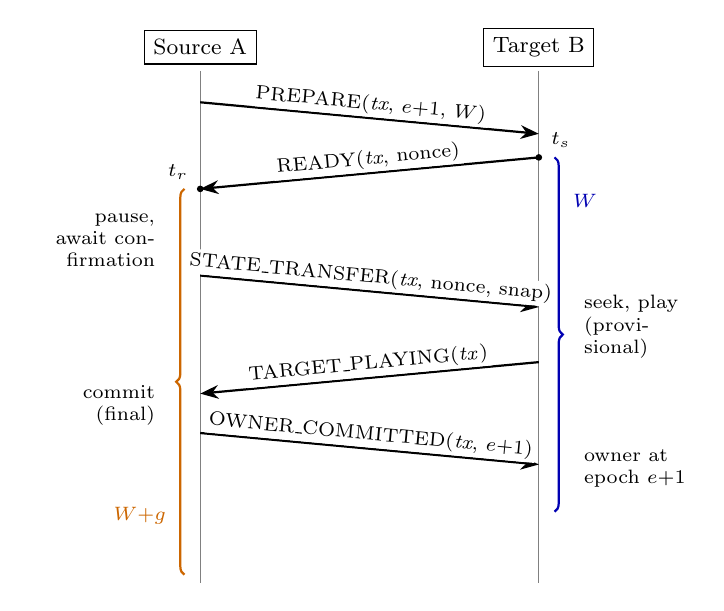
\begin{tikzpicture}[>=Stealth, font=\scriptsize,
  msg/.style={->, thick},
  lab/.style={fill=white, inner sep=1pt}]
  \def\xa{0} \def\xb{4.3}
  \node[draw, minimum width=1.4cm, font=\footnotesize] at (\xa,0) {Source A};
  \node[draw, minimum width=1.4cm, font=\footnotesize] at (\xb,0) {Target B};
  \draw[gray] (\xa,-0.3) -- (\xa,-6.8);
  \draw[gray] (\xb,-0.3) -- (\xb,-6.8);
  \draw[msg] (\xa,-0.7) -- node[lab, above, sloped] {PREPARE(\textit{tx}, $e{+}1$, $W$)} (\xb,-1.1);
  \draw[msg] (\xb,-1.4) -- node[lab, above, sloped] {READY(\textit{tx}, nonce)} (\xa,-1.8);
  \fill (\xb,-1.4) circle (1.2pt) node[above right=0pt and 1pt] {$t_s$};
  \fill (\xa,-1.8) circle (1.2pt) node[above left=0pt and 1pt] {$t_r$};
  \node[left, align=right, text width=1.5cm] at (\xa-0.45,-2.45) {pause, await confirmation};
  \draw[msg] (\xa,-2.9) -- node[lab, above, sloped] {STATE\_TRANSFER(\textit{tx}, nonce, snap)} (\xb,-3.3);
  \node[right, align=left, text width=1.3cm] at (\xb+0.45,-3.55) {seek, play (provisional)};
  \draw[msg] (\xb,-4.0) -- node[lab, above, sloped] {TARGET\_PLAYING(\textit{tx})} (\xa,-4.4);
  \node[left, align=right, text width=1.5cm] at (\xa-0.45,-4.55) {commit (final)};
  \draw[msg] (\xa,-4.9) -- node[lab, above, sloped] {OWNER\_COMMITTED(\textit{tx}, $e{+}1$)} (\xb,-5.3);
  \node[right, align=left, text width=1.3cm] at (\xb+0.45,-5.35) {owner at epoch $e{+}1$};
  \draw[decorate, decoration={brace, amplitude=3pt}, thick, blue!70!black] (\xb+0.2,-1.4) -- (\xb+0.2,-5.9)
    node[midway, right=3pt, rotate=0, yshift=17mm] {$W$};
  \draw[decorate, decoration={brace, amplitude=3pt, mirror}, thick, orange!80!black] (\xa-0.2,-1.8) -- (\xa-0.2,-6.7)
    node[midway, left=3pt, yshift=-17mm] {$W{+}g$};
\end{tikzpicture}
\caption{A successful handoff. B's window starts when B \emph{sends} READY ($t_s$); A's lease starts when A \emph{receives} it ($t_r \ge t_s$). B stops itself at the end of $W$ unless committed; A may abort only after $W+g$.}
\label{fig:seq}
\end{figure}

\begin{table}[t]
\caption{Protocol Messages}
\label{tab:msgs}
\centering
\footnotesize
\setlength{\tabcolsep}{4pt}
\begin{tabularx}{\columnwidth}{@{}>{\scriptsize\raggedright\arraybackslash}p{2.55cm}L{0.72cm}Y@{}}
\toprule
\textbf{Message} & \textbf{Dir.} & \textbf{Meaning} \\
\midrule
PREPARE & A$\to$B & Request handoff at a new epoch with window $W$ \\
READY & B$\to$A & B is idle, routed to the headset, window started; carries a nonce \\
REJECTED & B$\to$A & Stale epoch, not owner, busy, no route, or user override \\
STATE\_TRANSFER & A$\to$B & A is paused; play this content at this position; echoes nonce \\
TARGET\_PLAYING & B$\to$A & B plays provisionally \\
OWNER\_COMMITTED & A$\to$B & A committed; B owns the session \\
ABORT\_REQ & A$\to$B & Stop and confirm \\
ABORTED & B$\to$A & B is not playing \textit{tx} and never will \\
RECOVERY\_QUERY & B$\to$A & B has stopped uncommitted; asks for the decision \\
OWNER\_CLAIM & either & User pressed play here; new epoch \\
\bottomrule
\end{tabularx}
\end{table}

\subsection{Rules}

Let $t_s$ be the instant B sends READY, on B's timer, and $t_r$ the instant A receives it, on A's timer; $g$ is a guard.

\begin{itemize}
\item[R1] B starts playback only on a STATE\_TRANSFER that echoes its nonce and arrives before $t_s + W - b_{\mathrm{start}}$, and only with route evidence L2.
\item[R2] Unless it has received OWNER\_COMMITTED, B issues a pause at $t_s + W - b_{\mathrm{pause}}$; if its start is still pending then, it issues the pause as soon as the start completes. B never has two player commands outstanding. After the pause completes, B sends RECOVERY\_QUERY.
\item[R3] A takes the snapshot only after its own pause is confirmed.
\item[R4] A commits on the first TARGET\_PLAYING, or on a RECOVERY\_QUERY reporting that B had started, if either arrives before its lease expires at $t_r + W + g$; otherwise it decides abort. Either decision is final.
\item[R5] Under the \emph{rollback} policy A resumes when it decides abort. Under \emph{safe-pause} it resumes only on receiving ABORTED.
\item[R6] Each phone remembers finished transactions and rejects messages that refer to them.
\item[R7] Over every authenticated link, each phone announces its (owner, epoch) when the link comes up, on every change and every 5\,s. A peer's claim to own at a newer epoch is processed as that peer's OWNER\_CLAIM. If two idle phones claim the same epoch, the one that is playing (if both play, the one with the higher device identifier) claims a new epoch, and the other pauses on receiving it.
\end{itemize}

Our implementation uses $W=4$\,s, $g=0.5$\,s, $b_{\mathrm{start}}=1$\,s, $b_{\mathrm{pause}}=0.3$\,s and a 250\,ms retransmission interval. \draftnote{These values are provisional and will be set from measured P99 player latencies.}

\subsection{Safety Argument}

Assume B's coordinator runs, or restarts with its persisted state (R2 then executes on restart), and that the player meets P1--P3.

\textbf{Safe-pause.} Once it has sent STATE\_TRANSFER, A resumes only on ABORTED. B sends ABORTED only for a transaction it never started, or after its pause has completed: on ABORT\_REQ it first stops, letting a pending start complete and then pausing. By P1 and P3, no command issued before that pause produces audio afterwards. If A decides abort before sending any STATE\_TRANSFER, it may resume as soon as its own pause completes, because B cannot start without that message (R1, R3). A commit, by R4, is final and A never resumes after it. Neither case compares durations, so safety needs no bound on drift or latency; these affect only how long the phones stay silent.

\textbf{Rollback.} A resumes on a timer, so durations matter. Let $\delta$ bound the coordinator's reaction time to a player callback. Measured from $t_s$ in real time, B accepts a transfer no later than $(W-b_{\mathrm{start}})/(1-\rho)$ (R1); its start completes within $b_{\mathrm{start}}$ (P2); its pause is issued at the later of $(W-b_{\mathrm{pause}})/(1-\rho)$ and the start's completion, plus $\delta$, and completes within $b_{\mathrm{pause}}$ (R2, P3). A message is received after it is sent, so $t_r \ge t_s$, and A resumes no earlier than $(W+g)/(1+\rho)$ after $t_r$ unless it committed. The players cannot overlap if
\begin{equation}
\begin{split}
\frac{W+g}{1+\rho} > {} & \max\!\left(\frac{W-b_{\mathrm{start}}}{1-\rho} + b_{\mathrm{start}},\ \frac{W-b_{\mathrm{pause}}}{1-\rho}\right) \\
 & + \delta + b_{\mathrm{pause}}.
\end{split}
\label{eq:safety}
\end{equation}
With our parameters and $\rho = 100$\,ppm, the left side is 4.4996\,s and the right side $4.3003\,\mathrm{s} + \delta$, so (\ref{eq:safety}) holds for $\delta < 199$\,ms. Drift contributes less than 1\,ms; the guard is consumed by $b_{\mathrm{pause}}$ and scheduling delay, which is why its value must come from measured player latencies. The argument compares two durations that start at causally ordered events and never compares the phones' clocks. It adapts the lease of Gray and Cheriton~\cite{gray1989} to a two-party ownership transfer, with the holder's term starting when it sends READY and the grantor's when it receives it.

\textbf{Recovery.} A target that stopped uncommitted (R2) retransmits RECOVERY\_QUERY until A answers. A answers OWNER\_COMMITTED if it has committed; commits and answers so if its lease is still running, which is safe because B is already silent; and otherwise decides abort and answers ABORT\_REQ. On OWNER\_COMMITTED, B becomes the owner and resumes from its own paused position, which is where its content stopped; the cost is the silence in between. On ABORT\_REQ, B answers ABORTED and stays paused and not owner. A commit that reaches B while its pause is still in progress takes effect after the pause, followed by the same resume. Because A's decision is final and A never resumes after committing, B may act on a commit at any later time, including after its window; a commit never follows an abort decision. If the link does not return, B stays paused; A resumes after its lease under rollback and stays paused under safe-pause until the user presses play.

\textbf{The orphaned-player hazard.} If B's coordinator process dies inside the window and does not return before A's lease expires, R2 does not execute and the music app keeps playing. Under rollback, A then resumes while B plays. Under safe-pause, A stays silent until B restarts, pauses its player and answers. Section~\ref{sec:faulteval} measures both policies.

\textbf{Freshness.} Without the nonce of R1, a delayed PREPARE and STATE\_TRANSFER of an aborted transaction can arrive in order after A has resumed, and B would start. The nonce ties a transfer to the READY of the current attempt; R6 covers transactions B has already seen.

\textbf{User intent and concurrent claims.} A manual pause cancels a pending transaction and suspends automatic handoffs to that phone until the user plays or pulls playback there. A manual play claims a new epoch; the other phone pauses on receiving the claim. If both users press play while the phones cannot communicate, both play: each follows an explicit command, and no protocol can stop a phone it cannot reach, so the safety property excludes this case. R7 makes such conflicts converge once the phones reconnect. R7 is implemented in the engine of Section~\ref{sec:impl} and exercised by its tests; the simulator of Section~\ref{sec:faulteval} does not model concurrent claims.

% =====================================================================
\section{Security Layer}\label{sec:security}

The security layer treats Nearby Connections as an untrusted pipe and places identity, key agreement and replay protection above it. $H$ is SHA-256, $\Vert$ concatenation, and \textit{id} a device identifier derived from the hash of the identity key.

\textbf{Enrolment (G3, G6).} Each phone holds an ECDSA P-256 identity key in the Android keystore. Two phones enrol once, held by the same user, with a commit-then-reveal exchange of their identity keys $pk$ and 128-bit nonces $n$: A sends $c = H(\text{``SG2-commit''} \Vert pk_A \Vert n_A)$; B replies $pk_B \Vert n_B$; A reveals $pk_A \Vert n_A$ and B checks $c$. Both display the six-digit code obtained by reducing the first 63 bits of $H(\text{``SG2-sas''} \Vert pk_A \Vert pk_B \Vert n_A \Vert n_B)$ modulo $10^6$, and the user confirms that the codes match. A commits to its key and nonce before seeing $n_B$, and B reveals $n_B$ before seeing $n_A$, so an active attacker who substitutes either key cannot choose the resulting code and succeeds with probability about $10^{-6}$ per attempt; this is the commit-then-reveal argument for authentication by short authenticated strings~\cite{vaudenay2005}. The code authenticates the pair of identity keys, not a session key. After both confirmations the phones run the session handshake below over the same connection, accepting only the compared key; the roster is stored only if it succeeds. Because that handshake binds the transport token, a relay that forwards the enrolment verbatim across two connections shows matching codes but fails there (Section~\ref{sec:seceval}). The core also computes key fingerprints for comparison by QR code; the application does not yet offer that method.

\textbf{Session handshake (G5, G7).} For each transport connection the initiator I and responder R exchange $\textit{id}_I \Vert E_I \Vert n_I$, then $\textit{id}_R \Vert E_R \Vert n_R \Vert \sigma_R$, then $\sigma_I$, where $E$ are ephemeral P-256 public keys, $n$ 128-bit nonces, and $\sigma_R$ and $\sigma_I$ ECDSA signatures with the identity keys over ``resp''$\Vert th$ and ``init''$\Vert th$, with
$th = H(\text{``SG2-hs''} \Vert \textit{id}_I \Vert \textit{id}_R \Vert E_I \Vert E_R \Vert n_I \Vert n_R \Vert H(\tau))$.
Here $\tau$ is the raw authentication token that Nearby Connections derives for this connection and exposes for programmatic authentication~\cite{nearbydocs}. Because the transcript names both identities, the identity bound to the session is the one that signed, the property SIGMA~\cite{sigma2003} was designed to ensure; our exchange has not been formally verified. An attacker who terminates a separate connection with each victim holds two different tokens, so neither victim's signature verifies at the other, and no user comparison is needed. With HKDF-SHA-256~\cite{rfc5869}, $PRK = \mathrm{Extract}(n_I \Vert n_R, \mathrm{ECDH}(e_I, e_R))$, the direction keys are $\mathrm{Expand}(PRK, \text{``i2r''} \Vert th, 32)$ and $\mathrm{Expand}(PRK, \text{``r2i''} \Vert th, 32)$, and the session identifier $sid = \mathrm{Expand}(PRK, \text{``sid''} \Vert th, 16)$.

\textbf{Message protection (G1).} A frame is a version byte, a 64-bit sequence number $q$ and the AES-256-GCM ciphertext with a 128-bit tag, under the sender's direction key, with the 96-bit nonce $0^{32} \Vert q$ and associated data ``SG2''$\Vert sid \Vert \textit{id}_{\mathrm{sender}} \Vert \textit{id}_{\mathrm{recipient}} \Vert q$; sealing adds 25\,bytes. Each handshake derives fresh keys from fresh ephemeral keys and nonces, each direction has its own key, and $q$ starts at 0 and increments, so no key and nonce pair repeats. A session lasts as long as its transport connection; a restarted process holds no keys and must run a new handshake, so neither sequence numbers nor replay state are persisted, and $2^{64}$ frames cannot be reached within a session. The receiver keeps a 64-entry sliding window. It checks the window without changing it, verifies the tag, and only then marks $q$ as seen. A forgery cannot move the window, whatever sequence number it carries, so the desynchronisation of base paper~A has no counterpart. Separate direction keys make reflected frames fail. The 128-bit tag follows base paper~A's own recommendation of a longer tag.

\textbf{Identifiers (G2).} Nearby Connections involves three identifiers with different owners. The service identifier is supplied by the application and must uniquely identify the app~\cite{nearbydiscover}; it is the same on every Segue phone, so it can reveal that an Segue phone is near but not which one. The endpoint name is also supplied by the application: Segue advertises a 64-bit truncation of $\mathrm{HMAC}_{k_d}(\text{``SG2-adv''} \Vert \textit{epoch})$, where $k_d = \mathrm{HMAC}_{K}(\text{``SG2-dev''} \Vert \textit{id})$ for the group key $K$ shared at enrolment and the epoch index changes every 15 minutes. Members recompute each other's names and so learn which phone is advertising; without $K$, two epochs' names cannot be linked. The endpoint identifier is assigned by Nearby Connections; how it is chosen and rotated, and how the service identifier appears on the air, are outside the application's control and have not been measured. Sequence numbers exist only inside the encrypted link.

\textbf{Route and proximity (G8).} Reachability is never treated as nearness. B answers READY and accepts STATE\_TRANSFER only with route evidence L2 (\texttt{AudioManager.getAudioDevicesForAttributes} for media~\cite{androidaudiomanager}, available from Android~13; on Android~12 only L1 is available), which places B within Bluetooth range of the headset. The reference player reports a start as successful only with L3 (\texttt{AudioTrack.getRoutedDevice}~\cite{androidaudiotrack}) and otherwise stops and reports failure, which aborts the handoff; for third-party players L3 is not observable. All deadlines are short relative windows that bound the age of a relayed message.

\textbf{Residual risk.} A relay that forwards a single connection at the radio layer preserves the token and passes the handshake; distance bounding would be needed to stop it. Such an attacker can delay and drop messages but cannot read, forge or replay them, and by Section~\ref{sec:protocol} delay and loss do not cause dual playback.

% =====================================================================
\section{Implementation}\label{sec:impl}

\textbf{Core.} The protocol and security layer form a dependency-free Kotlin module of 1{,}052 lines. Since the simulation was first reported, the module gained a state export and import for persistence, the hook that lifts a manual-pause suspension when the user pulls playback, and one fix found by the automated test campaign described below: a target that crashed after stopping, before its player had started, resumed its player's stale position when it later committed, rather than the transferred snapshot. The full simulation was re-run with the fixed module; 24 of its 120 rows changed by one or two attempts, the pooled dual-playback counts and every value in Tables~\ref{tab:default}--\ref{tab:silence} and Fig.~\ref{fig:ablation} are unchanged, and the released results are the re-run's output. The coordinator is a deterministic state machine of ten phases that reaches the outside world through an environment (monotonic time, timers, send), a player port (asynchronous pause and play with completion callbacks, and a snapshot) and a route predicate, so the coordinator evaluated in the simulator is the code that runs on the phone. A state-transfer message is 110\,bytes encoded and 135\,bytes sealed.

\textbf{Engine.} A second pure-Kotlin module (2{,}219 lines) runs the coordinator on real links. It carries the handshake and channel over a transport interface, implements enrolment, R7, and binds every protocol message's sender to the authenticated identity of the link it arrived on, since the coordinator trusts the sender field. It persists coordinator state write-ahead: messages and player commands emitted while an event is handled are held until the state has been synced to storage. It records the boot count with the state and, after a reboot, when \texttt{elapsedRealtime} restarts, treats the stored lease anchor as expired. An end-to-end test harness runs two or three simulated phones on a virtual clock over this engine with the real cryptography and coordinator; its 90 checks cover enrolment, relay attempts during enrolment and reconnection, handoff, pull and claim, replay and tampering, a target killed in the provisional window and restarted from files, a source rebooted while transferring, concurrent claims, a target player slower than $b_{\mathrm{start}}$, a complete run of the automated campaign below against ground truth, and reconnection when, as with Nearby, discovery reports each advertiser once per session and may see only one direction. Concurrent claims made while partitioned converged 280\,ms after reconnection, and claims made at the same instant over a live link converged in 370\,ms, with modelled latencies of 20\,ms per message.

\textbf{Android application.} The application (1{,}958 lines) hosts the engine in a foreground service of type \texttt{connectedDevice}, binds the transport to Nearby Connections, keeps the identity key in the Android keystore, implements the L2 and L3 route checks, and plays a test signal through an \texttt{AudioTrack} reference player that meets P1--P3 by construction (one control thread; a start timeout below $b_{\mathrm{start}}$; pause and flush before reporting). Every protocol event is logged with monotonic timestamps, and logs from two phones are aligned with clock-offset samples from periodic pings, with error at most half the round-trip time; on the engine tests' logs the alignment recovered the true gap and latency exactly. \textbf{Test campaign.} For the device experiments the engine carries a test mode, off by default and refused by a peer that has not enabled it, in which one phone conducts a scripted campaign over the authenticated link. Each case puts playback on a chosen source, arms faults on either phone (dropped, delayed or duplicated message types; a forced route failure; a link outage; a coordinator crash at a chosen phase, with the player left running), triggers a handoff, pull or claim, and records the expected and observed outcome in both logs. The cases cover normal handoffs in both directions, each message-loss and crash case of Section~\ref{sec:faulteval}, rejection paths, outages in the transfer and provisional windows, and concurrent claims, under both rollback policies. Logs, configuration and device information are exported as one archive per phone, and an analysis script aligns two or three archives and classifies every interval of overlapping playback as unexpected, an expected rollback hazard, or the consequence of both users pressing play. A continuous-integration workflow in the repository runs the protocol and engine tests, re-runs the simulation of Section~\ref{sec:faulteval} and compares its output byte for byte with the released results, and builds the application against the Android SDK and Nearby Connections library. \draftnote{The application has been installed and paired on the test devices, but no measurements have been made.}

\textbf{Spotify adapter.} A second player drives the Spotify app through the App Remote SDK. When one account is signed in on both phones, Spotify Connect makes each phone's app report the same session, and a command sent to either app acts on the active device; the SDK does not say which device that is. The adapter therefore treats playback as local only while Spotify is not paused and the phone is producing media audio, sends a pause only in that state, and starts by asking Spotify to make the phone the active device, which carries track, position and queue; with different accounts it starts the track by its identifier and seeks. Play and pause made in the Spotify app are reported to the engine as a claim and a status change. Spotify answers more slowly than the reference player, so this mode uses $W=10$\,s, $b_{\mathrm{start}}=5$\,s and $b_{\mathrm{pause}}=1.5$\,s, and a phone in the other mode refuses the transferred state. Pause completion here is Spotify's reported state, not an observation of the audio path, so P3 holds only as far as that report is accurate. The adapter's logic is tested against a model of this behaviour (same account and different accounts); \draftnote{it has not yet run against the Spotify app.} Its use is limited by Spotify's February 2026 Development Mode rules, which require the developer to hold Premium and cap each app at five authorised users~\cite{spotify2026}, and by the SDK's requirement of a Premium account to play a single track~\cite{spotifysdk}.

% =====================================================================
\section{Evaluation by Fault Injection}\label{sec:faulteval}

\textbf{Method.} A discrete-event simulator drives two coordinators, two players and a lossy link. Each trial makes three handoff attempts spaced 22\,s apart plus a random offset of up to 2\,s. A checkpoint 16\,s after each trigger records which phones play; if not exactly one, a simulated user presses play on the target. Trials use distinct seeds. For a given seed every variant sees the same outage, crash and clock schedule; per-message loss and delay are drawn as messages are sent and therefore differ between variants. Table~\ref{tab:runs} lists the 24 settings. Every variant, including A2$^-$, ran 50{,}000 trials (150{,}000 attempts) per setting: $5 \times 24 \times 150{,}000 = 18{,}000{,}000$ attempts, of which 17{,}999{,}696 started; 304 A0 attempts found the phones not in a one-player state at the trigger and were skipped.

\begin{table}[t]
\caption{Simulation Settings (Each Run by All Five Variants)}
\label{tab:runs}
\centering
\footnotesize
\begin{tabularx}{\columnwidth}{@{}lcY@{}}
\toprule
\textbf{Group} & \textbf{Settings} & \textbf{Swept (others at default)} \\
\midrule
Fault-free & 1 & No loss, skew, outage or crash \\
Loss & 6 & Loss 0, 2, 5, 10, 20, 30\% \\
Skew & 6 & Skew 0, 0.5, 1, 2, 5, 10\,s; no outage or crash \\
Outage & 4 & Probability 0, 5, 10, 20\%; no crash \\
Crash & 4 & Probability 0, 2, 5, 10\%; no outage \\
Crash role & 2 & 10\%, source only or target only \\
Stress & 1 & 10\% loss, 10\% outage, 30\% slow, 30\% duplicated \\
\midrule
Total & 24 & 23 fault settings; 1.15 million trials per variant \\
\bottomrule
\end{tabularx}
\end{table}

\textbf{Fault model.} Loss is independent per message. Delay is log-normal with a 30\,ms median, and 3\% of messages take an extra 0.5--6\,s; 3\% are duplicated and 1\% are duplicated again after 5--40\,s. An outage lasts 1.5--12\,s and starts within 1.5\,s of the trigger. A coordinator crash starts within 3\,s of the trigger and lasts 2--8\,s, with the player keeping its state. Wall clocks are offset uniformly within the skew bound and timers drift by up to 100\,ppm. Player commands take 30--300\,ms and 5\% of target starts fail. Unless swept, loss is 5\%, skew $\pm$1\,s, outage probability 10\% and crash probability 2\% per phone.

\textbf{Variants.} A0 pauses, transfers and rolls back on an acknowledgement timeout. A1 adds PREPARE/READY, owner epochs, finished-transaction memory and a wall-clock expiry; its target commits on start, and conflicts are reconciled by epoch. A2 is the protocol of Section~\ref{sec:protocol} with rollback, A3 with safe-pause, and A2$^-$ is A2 without the nonce and transaction memory.

\begin{table}[t]
\caption{Default Fault Setting (150{,}000 Attempts per Variant)}
\label{tab:default}
\centering
\footnotesize
\setlength{\tabcolsep}{3.2pt}
\begin{tabular}{@{}lcccccc@{}}
\toprule
 & \multicolumn{4}{c}{\textbf{State at checkpoint (\%)}} & \textbf{Dual} & \textbf{Both} \\
\cmidrule(lr){2-5}
\textbf{Variant} & \textbf{Target} & \textbf{Source} & \textbf{Neither} & \textbf{Both} & \textbf{(\%)} & \textbf{owner} \\
\midrule
A0 naive & 92.00 & 6.44 & 0.051 & 1.503 & 1.503 & 2{,}247 \\
A1 expiry & 92.62 & 7.38 & 0 & 0 & 1.152 & 0 \\
A2 lease, rollback & 91.44 & 8.56 & 0 & 0 & 0.089 & 0 \\
A3 lease, safe-pause & 91.43 & 8.57 & 0 & 0 & 0 & 0 \\
\bottomrule
\end{tabular}
\\[2pt]
\parbox{\columnwidth}{\scriptsize The four checkpoint states partition the started attempts (149{,}993 for A0, whose 7 skipped attempts are excluded; 150{,}000 otherwise). Dual: attempts with $\ge$100\,ms of simultaneous playback at any time before the checkpoint, so A1 and A2 overlaps that ended before it are counted here but not under Both. Both owner: attempts ending with both coordinators believing they own the session. P99 silence was 3.18, 4.60, 4.46 and 7.46\,s for A0--A3.}
\end{table}

\begin{table}[t]
\caption{Dual Playback Pooled over the 23 Fault Settings}
\label{tab:pooled}
\centering
\footnotesize
\begin{tabular}{@{}lrrr@{}}
\toprule
\textbf{Variant} & \textbf{Attempts} & \textbf{With dual (\%)} & \textbf{Trials with dual} \\
\midrule
A0 naive & 3{,}449{,}696 & 29{,}526 (0.856) & 28{,}931 \\
A1 expiry & 3{,}450{,}000 & 22{,}397 (0.649) & 22{,}128 \\
A2 lease, rollback & 3{,}450{,}000 & 2{,}191 (0.064) & 2{,}188 \\
A2$^-$ without freshness & 3{,}450{,}000 & 2{,}547 (0.074) & 2{,}544 \\
A3 lease, safe-pause & 3{,}450{,}000 & 0 (0) & 0 \\
\bottomrule
\end{tabular}
\\[2pt]
\parbox{\columnwidth}{\scriptsize 1{,}150{,}000 trials per variant. The abstract's percentages are this table's A0 and A1 rows.}
\end{table}

\begin{figure*}[t]
\centering
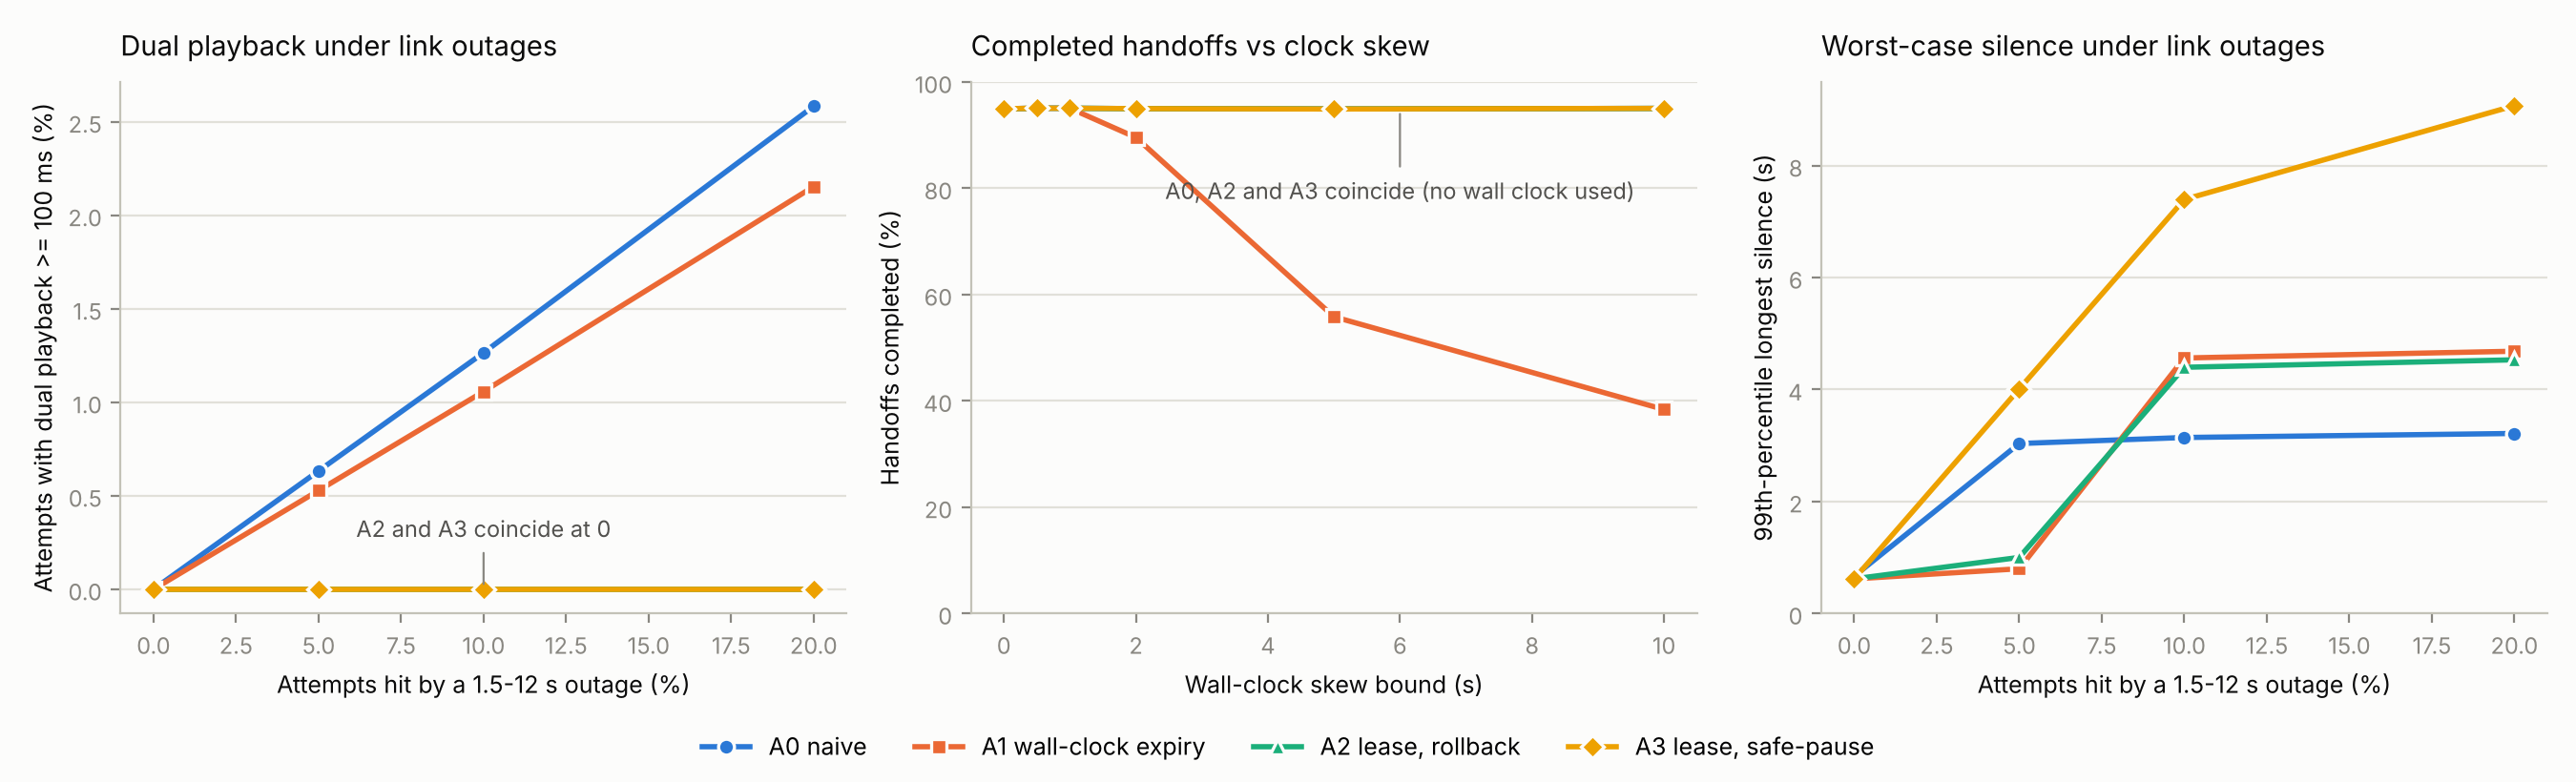
\includegraphics[width=\textwidth]{fig_ablation.png}
\caption{Ablation over 150{,}000 attempts per point. Left: dual playback against outage probability (no crashes); A2 and A3 coincide at zero. Centre: completed handoffs against wall-clock skew (no outages or crashes). Right: 99th-percentile longest silence per attempt against outage probability. The plotted values are in the released CSV.}
\label{fig:ablation}
\end{figure*}

\begin{table}[t]
\caption{Dual Playback (\% of Attempts) vs. Coordinator Crashes, No Outages}
\label{tab:crash}
\centering
\footnotesize
\begin{tabular}{@{}lcccc@{}}
\toprule
\textbf{Crash probability per phone} & \textbf{A0} & \textbf{A1} & \textbf{A2} & \textbf{A3} \\
\midrule
0\% & 0 & 0 & 0 & 0 \\
2\% & 0.258 & 0.149 & 0.067 & 0 \\
5\% & 0.693 & 0.385 & 0.175 & 0 \\
10\% & 1.409 & 0.827 & 0.359 & 0 \\
10\%, source only & 0.768 & 0.479 & 0 & 0 \\
10\%, target only & 0.615 & 0.357 & 0.350 & 0 \\
\bottomrule
\end{tabular}
\end{table}

\begin{table}[t]
\caption{Longest Silence per Attempt (s) vs. Outage Probability}
\label{tab:silence}
\centering
\footnotesize
\begin{tabular}{@{}lcccc@{}}
\toprule
\textbf{Outage probability} & \textbf{A2 P95} & \textbf{A3 P95} & \textbf{A2 P99} & \textbf{A3 P99} \\
\midrule
0\% & 0.48 & 0.48 & 0.62 & 0.62 \\
5\% & 0.51 & 0.51 & 1.00 & 4.01 \\
10\% & 0.55 & 0.55 & 4.40 & 7.40 \\
20\% & 0.82 & 2.45 & 4.53 & 9.07 \\
\bottomrule
\end{tabular}
\end{table}

\textbf{Results.} Without faults every variant completed all 150{,}000 attempts. Table~\ref{tab:default} gives the default setting, Table~\ref{tab:pooled} the totals over all fault settings, Fig.~\ref{fig:ablation} the outage and skew sweeps, and Tables~\ref{tab:crash} and~\ref{tab:silence} the crash and silence results.

\begin{enumerate}
\item \emph{Safety.} A3 had no dual playback in 3{,}450{,}000 attempts, or 1{,}150{,}000 trials, across the 23 fault settings. The three attempts of a trial share state, so we bound per trial rather than per attempt: zero of 1{,}150{,}000 trials gives a 95\% upper bound of $2.6\times10^{-6}$ on the probability that a trial drawn from the pooled settings contains any dual playback (rule of three), and for any single setting the bound is $6.0\times10^{-5}$ (zero of 50{,}000 trials). These bounds hold only under the simulated fault model. A2 had none in the 1{,}950{,}000 attempts of the 13 settings without target-coordinator crashes and 2{,}191 in the other ten.
\item \emph{The hazard is the orphaned player.} With crashes confined to the source, A2 had no dual playback; confined to the target, 0.350\% (Table~\ref{tab:crash}). The longest overlap observed for A2 was 5.8\,s.
\item \emph{Expiry and rollback do not compose.} A1's dual playback grew with outage probability, from 0.528\% at 5\% to 2.153\% at 20\% (Fig.~\ref{fig:ablation}, left): the target has started, its report cannot reach the source, and the source's expiry fires.
\item \emph{Wall-clock deadlines fail availability first.} A1 completed 89.58\%, 55.83\% and 38.38\% of handoffs at $\pm$2, $\pm$5 and $\pm$10\,s skew, against 94.9--95.0\% for A2 and A3 (Fig.~\ref{fig:ablation}, centre); no variant from A0 to A3 showed dual playback in this sweep.
\item \emph{Freshness binding is necessary.} In the stress setting, A2$^-$ had dual playback in 325 of 150{,}000 attempts and A2 in none; pooled over all fault settings A2$^-$ had 356 more than A2 (Table~\ref{tab:pooled}).
\item \emph{Price of the lease.} Under outages A2 and A3 completed 0.5--2.2 percentage points fewer handoffs than A1, because a target that cannot confirm the commit stops and the source keeps the session. Safe-pause adds silence in the tail (Table~\ref{tab:silence}) and nothing at the median.
\end{enumerate}

Four A2 and five A3 attempts in 3.45 million each ended with neither phone playing at the checkpoint, all in settings with injected crashes. The silence values follow from the assumed player and link delays and are not audible-gap measurements; outage and crash probabilities are parameters, not field estimates. Simulation over random schedules is evidence, not proof.

% =====================================================================
\section{Security Evaluation}\label{sec:seceval}

Table~\ref{tab:sec} lists adversarial tests against the implemented layer. No forged, tampered, replayed or reflected frame and no relay across two transport connections was accepted in 2{,}308{,}000 attempts, and the 2{,}000 untampered originals were still delivered after 100{,}000 tampering attempts, showing that rejected input does not disturb receiver state. Relays that forward a single connection at the radio layer were not tested and are not stopped (Section~\ref{sec:security}). The engine tests add the enrolment case: a relay forwarding enrolment verbatim across two connections produced matching codes on both phones, and the binding handshake then failed and nothing was stored.

\begin{table}[t]
\caption{Adversarial Tests Against the Security Layer}
\label{tab:sec}
\centering
\footnotesize
\begin{tabularx}{\columnwidth}{@{}Yrrl@{}}
\toprule
\textbf{Test} & \textbf{Attempts} & \textbf{Accepted} & \textbf{Gap} \\
\midrule
Handshake, honest enrolled phones & 500 & 500 & -- \\
Outsider impersonates initiator & 500 & 0 & G5, G6 \\
Outsider impersonates responder & 500 & 0 & G5, G6 \\
Relay across two transport connections & 500 & 0 & G7 \\
One flipped bit in any handshake message & 500 & 0 & G5 \\
Random forged frames & 200{,}000 & 0 & G1 \\
Single-bit tamper of valid frames & 100{,}000 & 0 & G1 \\
Replay of every earlier frame & 2{,}000 & 0 & G1 \\
Reflection to sender & 2{,}000 & 0 & G1 \\
Replay into a new session & 2{,}000 & 0 & G1 \\
Near-maximum sequence-number forgeries & 2{,}000{,}000 & 0 & G1 \\
Legitimate frames after that flood & 1{,}000 & 1{,}000 & G1 \\
Legitimate frames reordered in window & 640 & 640 & -- \\
\bottomrule
\end{tabularx}
\end{table}

\textbf{Reproducing the desynchronisation class.} To confirm that our tests can detect gap G1, we built a deliberately weak channel that accepts only a counter higher than the last accepted one, authenticated by a truncated tag. It is a generic design, not a model of Apple's implementation. An attacker without the key sends a maximum counter and enumerates tag values. Table~\ref{tab:desync} shows that the cost doubles with each tag bit and that a successful attack blocks all later legitimate frames; with an 8-bit tag no run needed more than 256 forgeries, the number base paper~A reports for Handoff's 1-byte tag.

\begin{table}[t]
\caption{Forgeries to Desynchronise a Higher-Counter-Only Channel}
\label{tab:desync}
\centering
\footnotesize
\begin{tabular}{@{}lrrrr@{}}
\toprule
\textbf{Tag} & \textbf{Trials} & \textbf{Mean} & \textbf{Max.} & \textbf{Legit.\ delivered after} \\
\midrule
8 bit & 200 & 123 & 253 & 0 / 20{,}000 \\
12 bit & 200 & 2{,}186 & 4{,}083 & 0 / 20{,}000 \\
16 bit & 200 & 33{,}553 & 65{,}374 & 0 / 20{,}000 \\
20 bit & 40 & 570{,}769 & 1{,}035{,}767 & 0 / 4{,}000 \\
\bottomrule
\end{tabular}
\end{table}

\textbf{Cost.} On a two-vCPU cloud virtual machine (JDK~21), sealing and opening one message took 0.9--1.3\,\textmu s and a full handshake 3.2--4.3\,ms across two runs. \draftnote{Phone measurements are in Table~\ref{tab:hw}.}

% =====================================================================
\section{Device Evaluation (In Progress)}\label{sec:hw}

\draftnote{No phone or headset measurements have been made. Every cell marked \tbm\ must be filled from logged runs before submission.}

\textbf{Setup.} Primary pair: two phones, a vivo X80 (Funtouch~OS, Android~15) and an iQOO~7 (Funtouch~OS, Android~13). Secondary pair: the X80 and a OnePlus Pad~3 tablet (OxygenOS~16, Android~16). During each pair's runs the third device stays enrolled and connected and must neither play nor lose track of the owner. Exact builds \tbm. Headset: realme Buds Air~8 (Bluetooth~5.4, three-device multipoint, SBC/AAC/LHDC); firmware and codec in use \tbm. Player: the reference player of Section~\ref{sec:impl}; Spotify App Remote for up to five accounts once its adapter exists. Transport: Nearby Connections with the layer of Section~\ref{sec:security}.

\textbf{Instruments.} The reference player's test signal is a pure function of content position: a quiet 220\,Hz tone and, at the start of every content second, a 60\,ms chirp whose pitch encodes the second. A microphone recording of one earbud gives the audible gap as the silent stretch of the tone and the position error from the spacing of the chirps around it. Each edge is placed where that side's own tone energy falls to the half-overlap level, so a volume difference between the phones does not bias the result. On synthetic recordings with known gaps of 250--410\,ms, position errors of $-40$ to $+100$\,ms and a 6\,dB level change, the analysis was within $\pm$2\,ms. Phone-side intervals come from the two event logs aligned by the ping-based clock offsets.

\begin{table}[t]
\caption{Device Measurements, Phone Pair (200 Handoffs per Direction)}
\label{tab:hw}
\centering
\footnotesize
\begin{tabular}{@{}lcccc@{}}
\toprule
 & \multicolumn{2}{c}{\textbf{A$\to$B}} & \multicolumn{2}{c}{\textbf{B$\to$A}} \\
\textbf{Metric} & \textbf{Med.} & \textbf{P95} & \textbf{Med.} & \textbf{P95} \\
\midrule
Audible gap, microphone (ms) & \tbm & \tbm & \tbm & \tbm \\
Position error, microphone (ms) & \tbm & \tbm & \tbm & \tbm \\
Request to target audio started (ms) & \tbm & \tbm & \tbm & \tbm \\
Source paused to target started (ms) & \tbm & \tbm & \tbm & \tbm \\
Player start latency (ms) & \tbm & \tbm & \tbm & \tbm \\
Player pause latency (ms) & \tbm & \tbm & \tbm & \tbm \\
Handshake (ms) & \tbm & \tbm & \tbm & \tbm \\
\midrule
Dual playback events, $\ge$500 runs & \multicolumn{4}{c}{\tbm} \\
Battery, 4\,h listening (mAh/h) & \multicolumn{4}{c}{\tbm} \\
\bottomrule
\end{tabular}
\end{table}

The phone--tablet pair is measured the same way and reported in a second table \tbm. The device campaign will also measure the player latencies that fix $b_{\mathrm{start}}$, $b_{\mathrm{pause}}$ and $g$ through (\ref{eq:safety}), inject message drops, link loss, coordinator kills on each phone and Doze conditions (at least 150 faulty runs), compare the result with the simulator at the measured loss and delay, and time the same handoff done manually, through vendor audio switching where the headset supports it, and, where Android~17 Continue On supports the device pair, through it.

% =====================================================================
\section{Discussion and Limitations}

The central trade-off is availability for safety: the lease gives up a few percent of completed handoffs under outages, and safe-pause adds seconds of silence in the worst cases, in exchange for never playing on both phones.

\textbf{Simulation and engine tests, not devices.} All protocol results come from a chosen fault model and from engine tests with modelled latencies. The guarantee concerns player states; it holds on a phone only if the player meets P1--P3 and, for rollback, if measured latencies satisfy (\ref{eq:safety}). The reference player enforces P2 with a start timeout; a third-party player can be held to its pause budget only as far as its API reports completion. Real headsets may delay stream switching or refuse to switch, which would limit the product but not the property.

\textbf{Vendor audio switching.} Where Apple's, Samsung's or Google's switching applies, much of the manual effort already disappears~\cite{applesw,samsungsw,googlesw}. Segue targets multipoint earbuds and phones without a shared vendor account, moves the session and its position instead of waiting for the user to start playback on the second phone, and states and tests its behaviour under faults. Whether users prefer it is a question for the planned pilot.

\textbf{Process death.} Safe-pause is safe only if the restarted target pauses before answering, which needs persisted state and a foreground service; the engine persists write-ahead, but Android may not restart the service by itself. If it never restarts, the target plays until the user intervenes while the source stays silent: one player, but not necessarily the intended one.

\textbf{Other limits.} Radio-layer relays are not stopped (Section~\ref{sec:security}); a stolen enrolled phone can issue handoffs until removed from the roster; control of third-party players is limited to what each player's API exposes and can change without notice, as Spotify's 2026 developer changes illustrate~\cite{spotify2026}; and each transaction involves two devices: other enrolled devices learn the new owner through R7, but neither the simulator nor the safety argument covers more than two. Android~17's Continue On~\cite{android17,continueon} requires each app to opt in and initially targets phone-to-tablet transitions, but it may expand and overlap with the application, so our claims rest on the exclusive-ownership protocol without clock synchronisation, the orphaned-player analysis and the security layer. The safety argument is informal; model checking is future work.

% =====================================================================
\section{Conclusion}

Automatic playback handoff between two phones can be made exclusive without synchronised clocks by anchoring a provisional lease on the target's READY and letting only the source decide; with safe-pause rollback, exclusivity of player states needs no timing assumption at all. Across 18.0 million simulated attempts, this lease with safe-pause rollback and freshness binding eliminated the dual playback that expiry-based and naive designs produced, and wall-clock deadlines failed under skew long before they failed safety. The security layer closes the application-reachable gaps of two published analyses and resisted 2.3 million adversarial attempts. The device campaign of Section~\ref{sec:hw} will determine whether the player contract and these results carry over to real phones and headsets.

\section*{Artifact Availability}
The Kotlin core, engine, Android application, simulator, raw results, analysis scripts and this paper's sources are available at \url{https://github.com/Keshav-gehlot/Segue}. \draftnote{An archival DOI will be added on release.}

% ---------------------------------------------------------------------
% References. Order is generated by first citation (see sort_refs.py).
% All entries were checked against publisher, index or official pages on 16 Nov 2026.
\begin{thebibliography}{99}

\bibitem{applesw}
Apple, ``Switch your AirPods to another device,'' Apple Support, article 104988. Accessed: Nov. 16, 2026. [Online]. Available: \url{https://support.apple.com/104988}

\bibitem{samsungsw}
Samsung, ``Use Auto switch with your Galaxy buds and paired devices,'' Samsung US Support. Accessed: Nov. 16, 2026. [Online]. Available: \url{https://www.samsung.com/us/support/answer/ANS10002627/}

\bibitem{googlesw}
A.~Hsiao, ``How we're helping you switch audio between devices,'' \emph{The Keyword} (Google), Jul. 21, 2022. [Online]. Available: \url{https://www.blog.google/products/android/better-together-audio-switching/}

\bibitem{stute2021}
M.~Stute, A.~Heinrich, J.~Lorenz, and M.~Hollick, ``Disrupting continuity of Apple's wireless ecosystem security: New tracking, DoS, and MitM attacks on iOS and macOS through Bluetooth Low Energy, AWDL, and Wi-Fi,'' in \emph{Proc. 30th USENIX Security Symp.}, 2021, pp. 3917--3934.

\bibitem{android17}
Google, ``The second beta of Android 17,'' \emph{Android Developers Blog}, Feb. 26, 2026. [Online]. Available: \url{https://android-developers.googleblog.com/2026/02/the-second-beta-of-android-17.html}

\bibitem{continueon}
Google, ``About the Continue On feature,'' Android Developers. Accessed: Nov. 16, 2026. [Online]. Available: \url{https://developer.android.com/develop/better-together/continue-on}

\bibitem{antonioli2019}
D.~Antonioli, N.~O. Tippenhauer, and K.~Rasmussen, ``Nearby threats: Reversing, analyzing, and attacking Google's `Nearby Connections' on Android,'' in \emph{Proc. Netw. Distrib. Syst. Secur. Symp. (NDSS)}, San Diego, CA, USA, 2019.

\bibitem{bias2020}
D.~Antonioli, N.~O. Tippenhauer, and K.~Rasmussen, ``BIAS: Bluetooth impersonation attacks,'' in \emph{Proc. IEEE Symp. Secur. Privacy (SP)}, 2020, pp. 549--562.

\bibitem{bluffs2023}
D.~Antonioli, ``BLUFFS: Bluetooth forward and future secrecy attacks and defenses,'' in \emph{Proc. ACM SIGSAC Conf. Comput. Commun. Secur. (CCS)}, Copenhagen, Denmark, 2023, doi: 10.1145/3576915.3623066.

\bibitem{blurtooth2020}
D.~Antonioli, N.~O. Tippenhauer, K.~Rasmussen, and M.~Payer, ``BLURtooth: Exploiting cross-transport key derivation in Bluetooth Classic and Bluetooth Low Energy,'' in \emph{Proc. ACM Asia Conf. Comput. Commun. Secur. (ASIA CCS)}, Nagasaki, Japan, 2022, pp. 196--207.

\bibitem{happymitm2021}
J.~Classen and M.~Hollick, ``Happy MitM: Fun and toys in every Bluetooth device,'' in \emph{Proc. 14th ACM Conf. Secur. Privacy Wireless Mobile Netw. (WiSec)}, 2021, pp. 72--77.

\bibitem{stealtooth2025}
K.~Kimura, H.~Kuzuno, Y.~Shiraishi, and M.~Morii, ``Stealtooth: Breaking Bluetooth security abusing silent automatic pairing,'' 2025, \emph{arXiv:2507.00847}.

\bibitem{martin2019}
J.~Martin \emph{et al.}, ``Handoff all your privacy -- A review of Apple's Bluetooth Low Energy continuity protocol,'' \emph{Proc. Privacy Enhancing Technol.}, vol. 2019, no. 4, pp. 34--53, 2019.

\bibitem{heinze2020}
D.~Heinze, J.~Classen, and F.~Rohrbach, ``MagicPairing: Apple's take on securing Bluetooth peripherals,'' in \emph{Proc. 13th ACM Conf. Secur. Privacy Wireless Mobile Netw. (WiSec)}, 2020, doi: 10.1145/3395351.3399343.

\bibitem{fastpair}
Google, ``Google Fast Pair Service: Introduction,'' Nearby specifications. Accessed: Nov. 16, 2026. [Online]. Available: \url{https://developers.google.com/nearby/fast-pair/specifications/introduction}

\bibitem{quickshell2024}
O.~Yair and S.~Cohen, ``QuickShell: Sharing is caring about an RCE attack chain on Quick Share,'' presented at DEF CON 32, Las Vegas, NV, USA, Aug. 2024.

\bibitem{bison2023}
T.~Gasteiger, C.~A. Boano, and K.~R{\"o}mer, ``BISON: Attacking Bluetooth's broadcast isochronous streams,'' in \emph{Proc. Int. Conf. Embedded Wireless Syst. Netw. (EWSN)}, 2023, pp. 256--261.

\bibitem{shacham2007}
R.~Shacham, H.~Schulzrinne, S.~Thakolsri, and W.~Kellerer, ``Ubiquitous device personalization and use: The next generation of IP multimedia communications,'' \emph{ACM Trans. Multimedia Comput. Commun. Appl.}, vol. 3, no. 2, Art. no. 12, May 2007.

\bibitem{rfc5631}
R.~Shacham, H.~Schulzrinne, S.~Thakolsri, and W.~Kellerer, ``Session Initiation Protocol (SIP) session mobility,'' IETF RFC 5631, Oct. 2009.

\bibitem{flux2015}
A.~Van't Hof, H.~Jamjoom, J.~Nieh, and D.~Williams, ``Flux: Multi-surface computing in Android,'' in \emph{Proc. 10th Eur. Conf. Comput. Syst. (EuroSys)}, Bordeaux, France, 2015, doi: 10.1145/2741948.2741955.

\bibitem{baton2014}
``Handoff for Android: Nextbit announces backup and syncing service Baton,'' \emph{9to5Google}, Oct. 27, 2014. [Online]. Available: \url{https://9to5google.com/2014/10/27/handoff-for-android-nextbit-baton/}

\bibitem{deepshot2011}
T.-H. Chang and Y.~Li, ``Deep Shot: A framework for migrating tasks across devices using mobile phone cameras,'' in \emph{Proc. ACM CHI Conf. Human Factors Comput. Syst.}, 2011, pp. 2163--2172.

\bibitem{brudy2019}
F.~Brudy, C.~Holz, R.~R{\"a}dle, C.-J. Wu, S.~Houben, C.~N. Klokmose, and N.~Marquardt, ``Cross-device taxonomy: Survey, opportunities and challenges of interactions spanning across multiple devices,'' in \emph{Proc. ACM CHI Conf. Human Factors Comput. Syst.}, 2019, doi: 10.1145/3290605.3300792.

\bibitem{arora2015}
A.~Arora, D.~S. Goldstein, and D.~C. Hwang, ``Automated transition of content consumption across devices,'' U.S. Patent Appl. US 2015/0215382 A1, Jul. 30, 2015.

\bibitem{zhang2006}
J.~Zhang, ``Seamless multimedia session handoff across multiple devices in a mobile networking environment,'' Int. Patent Appl. WO 2006/028456 A1, Mar. 16, 2006.

\bibitem{trip2018}
B.~Trip, R.~Koops, E.~Klaassens, K.~Gallione, J.~B. Ledingham, and D.~de~Jong, ``Connection switching for Bluetooth headsets,'' U.S. Patent 9\,986\,370 B2, May 29, 2018.

\bibitem{gray1989}
C.~G. Gray and D.~R. Cheriton, ``Leases: An efficient fault-tolerant mechanism for distributed file cache consistency,'' in \emph{Proc. 12th ACM Symp. Operating Syst. Principles (SOSP)}, 1989, pp. 202--210.

\bibitem{chubby2006}
M.~Burrows, ``The Chubby lock service for loosely-coupled distributed systems,'' in \emph{Proc. 7th USENIX Symp. Operating Syst. Design Implementation (OSDI)}, 2006, pp. 335--350.

\bibitem{raft2014}
D.~Ongaro and J.~Ousterhout, ``In search of an understandable consensus algorithm,'' in \emph{Proc. USENIX Annu. Tech. Conf. (ATC)}, Philadelphia, PA, USA, 2014, pp. 305--319.

\bibitem{montagud2012}
M.~Montagud, F.~Boronat, H.~Stokking, and R.~van Brandenburg, ``Inter-destination multimedia synchronization: Schemes, use cases and standardization,'' \emph{Multimedia Syst.}, vol. 18, no. 6, pp. 459--482, 2012.

\bibitem{rfc7272}
R.~van Brandenburg, H.~Stokking, O.~van Deventer, F.~Boronat, M.~Montagud, and K.~Gross, ``Inter-destination media synchronization (IDMS) using the RTP Control Protocol (RTCP),'' IETF RFC 7272, Jun. 2014.

\bibitem{faragher2015}
R.~Faragher and R.~Harle, ``Location fingerprinting with Bluetooth Low Energy beacons,'' \emph{IEEE J. Sel. Areas Commun.}, vol. 33, no. 11, pp. 2418--2428, Nov. 2015.

\bibitem{leith2020}
D.~J. Leith and S.~Farrell, ``Measurement-based evaluation of Google/Apple Exposure Notification API for proximity detection in a commuter bus,'' \emph{PLoS ONE}, vol. 16, no. 4, Art. no. e0250826, 2021.

\bibitem{vaudenay2005}
S.~Vaudenay, ``Secure communications over insecure channels based on short authenticated strings,'' in \emph{Advances in Cryptology -- CRYPTO 2005}, LNCS, vol. 3621, 2005, pp. 309--326.

\bibitem{nearbydocs}
Google, ``ConnectionInfo,'' Google Play services API reference (Nearby Connections). Accessed: Nov. 16, 2026. [Online]. Available: \url{https://developers.google.com/android/reference/com/google/android/gms/nearby/connection/ConnectionInfo}

\bibitem{sigma2003}
H.~Krawczyk, ``SIGMA: The `SIGn-and-MAc' approach to authenticated Diffie-Hellman and its use in the IKE protocols,'' in \emph{Advances in Cryptology -- CRYPTO 2003}, LNCS, vol. 2729, 2003, pp. 400--425.

\bibitem{rfc5869}
H.~Krawczyk and P.~Eronen, ``HMAC-based extract-and-expand key derivation function (HKDF),'' IETF RFC 5869, May 2010.

\bibitem{nearbydiscover}
Google, ``Discover devices,'' Nearby Connections for Android. Accessed: Nov. 16, 2026. [Online]. Available: \url{https://developers.google.com/nearby/connections/android/discover-devices}

\bibitem{androidaudiomanager}
Google, ``AudioManager,'' Android API reference. Accessed: Nov. 16, 2026. [Online]. Available: \url{https://developer.android.com/reference/android/media/AudioManager}

\bibitem{androidaudiotrack}
Google, ``AudioTrack,'' Android API reference. Accessed: Nov. 16, 2026. [Online]. Available: \url{https://developer.android.com/reference/android/media/AudioTrack}

\bibitem{spotify2026}
Spotify, ``Update on developer access and platform security,'' \emph{Spotify for Developers} blog, Feb. 6, 2026. [Online]. Available: \url{https://developer.spotify.com/blog/2026-02-06-update-on-developer-access-and-platform-security}

\bibitem{spotifysdk}
Spotify, ``Spotify App Remote SDK (Android),'' Accessed: Nov. 16, 2026. [Online]. Available: \url{https://spotify.github.io/android-sdk/app-remote-lib}

\end{thebibliography}

\end{document}
